\section{Análisis de la precisión de los datos georreferenciados}

Con la finalidad de evaluar la precisión de los datos georreferenciados obtenidos a través de la aplicación móvil, se
desarrolló un prototipo de aplicación que permite obtener la ubicación del dispositivo móvil y compararla con un punto
de referencia conocido, el cual será seleccionado en la aplicación de prueba. Para ello, se utilizó el GPS del dispositivo
móvil para obtener la ubicación, el framework de desarrollo Flutter para la creación de la aplicación móvil y Google Maps
para la visualización de la ubicación en un mapa interactivo.
\bigbreak

En la Figura  \ref{fig:prototipo-georreferenciacion} se muestra el prototipo de la aplicación móvil desarrollada para la
evaluación de la precisión de los datos georreferenciados. Esta aplicación cuenta con un botón que permite obtener la ubicación
actual del dispositivo móvil. Con esto, el usuario puede seleccionar un punto de referencia en el mapa y guardar ambos puntos
para su posterior comparación.

\begin{figure}[H]
    \centering
    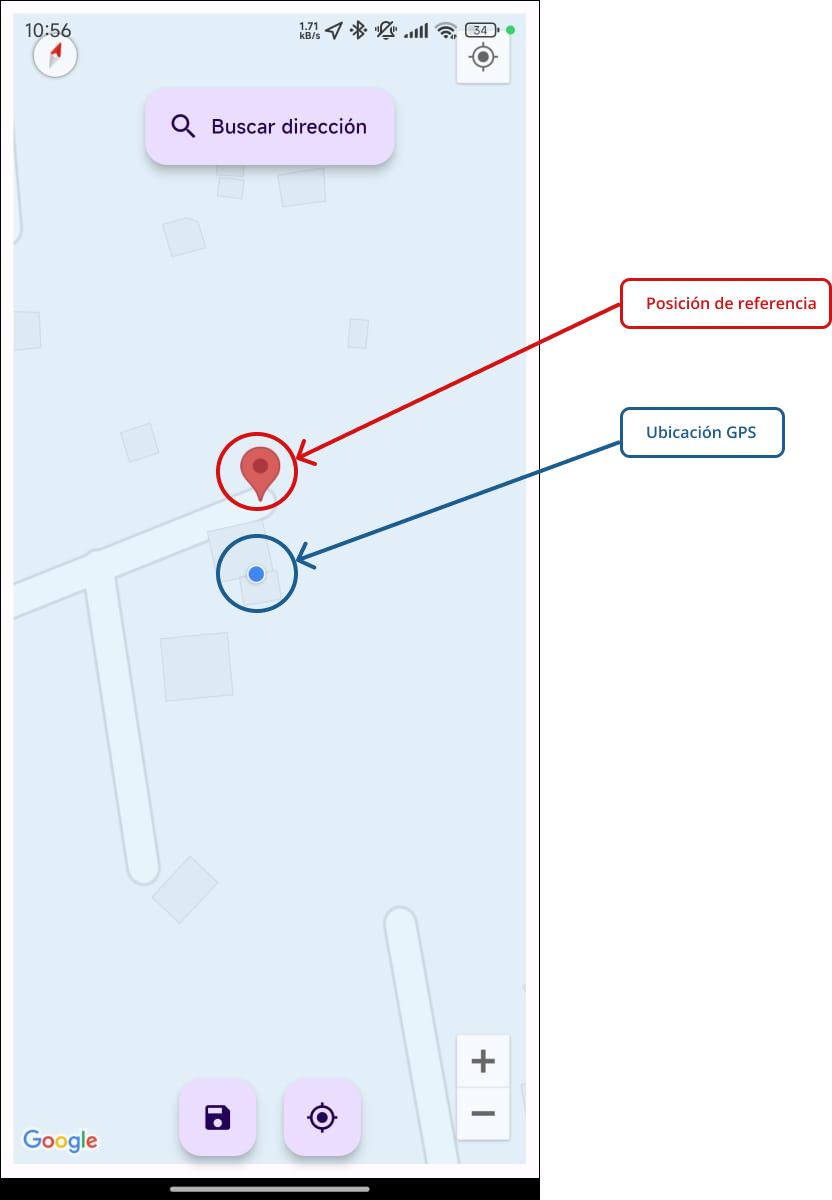
\includegraphics[width=0.3\textwidth]{chapters/III-resultados-y-discusion/resources/images/prototipo-georreferenciacion.png}
    \caption{Prototipo de la aplicación móvil para la evaluación de la precisión de los datos georreferenciados.}
    \label{fig:prototipo-georreferenciacion}
\end{figure}

Para establecer la cantidad de datos necesarios para la evaluación de la precisión de los datos georreferenciados, se optó por
utilizar una muestra infinita con población desconocida, aplicando la Ecuación \ref{eq:ecuacion-muestra-datos-georreferenciados},
donde:

\begin{itemize}
    \item n = tamaño de la muestra
    \item Z = nivel de confianza
    \item p = probabilidad de éxito o proporción esperada
    \item q = probabilidad de fracaso
    \item pq = varianza de la población
    \item e = error de estimación máximo aceptable
\end{itemize}

\begin{equation}
    n=\frac{Z^2 \cdot p \cdot q}{e^2}
    \label{eq:ecuacion-muestra-datos-georreferenciados}
\end{equation}

Sustituyendo los valores en la Ecuación \ref{eq:ecuacion-muestra-datos-georreferenciados}, se obtiene:

\begin{itemize}
    \item Z = 1.96, con un nivel de confianza del 95\% y un error de estimación máximo aceptable del 5\%
    \item p = 0.50
    \item q = 0.50
    \item e = 0.05
\end{itemize}

\begin{equation}
    n=\frac{(1.96)^2 \cdot 0.50 \cdot 0.50}{(0.05)^2}
    \label{eq:ecuacion-valores-muestra-datos-georreferenciados}
\end{equation}

\begin{equation}
    n=384.16 \approx 385
    \label{eq:ecuacion-resultado-muestra-datos-georreferenciados}
\end{equation}

Utilizando un nivel de confianza del 95\% y un error de estimación máximo aceptable del 5\%, se obtiene una muestra aproximada
de 385 puntos de referencia para la evaluación de la precisión de los datos georreferenciados.
\bigbreak

Los datos obtenidos de la aplicación móvil se almacenaron en una tabla de una base de datos PostgreSQL, la cual se muestra en
la Figura \ref{fig:tabla-georreferenciacion}. Esta tabla contiene la información de los puntos de referencia seleccionados en
la aplicación móvil, los cuales son: latitud y longitud real (Punto de referencia) y latitud y longitud obtenida mediante
GPS (Punto de ubicación).

\begin{figure}[H]
    \centering
    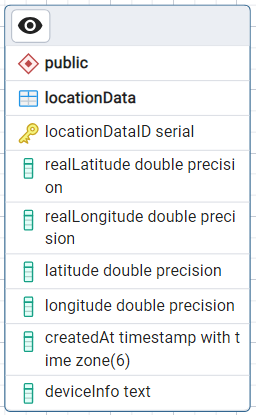
\includegraphics[width=0.3\textwidth]{chapters/III-resultados-y-discusion/resources/images/tabla-georreferenciacion.png}
    \caption{Tabla de datos georreferenciados almacenados en la base de datos PostgreSQL.}
    \label{fig:tabla-georreferenciacion}
\end{figure}

Estos datos se traspasaron a un archivo de Excel para su posterior análisis. Para ello, se utilizó un script con
Node.js y la librería de manejo de archivos ExcelJS, como se muestra en el Anexo \ref{apendix:script-exceljs}. La distancia entre
los puntos de referencia y los puntos de ubicación se calculó utilizando la fórmula de Haversine, dado que esta toma en cuenta
la curvatura de la Tierra y proporciona una mejor precisión \cite{basyirDeterminationNearestEmergency2017}. La función de
Haversine utilizada se muestra en el Anexo \ref{apendix:script-haversine}.

% \begin{figure}[H]
%     \begin{minted}[fontsize=\footnotesize, linenos, breaklines, frame=single]{js}
import Exceljs from "exceljs";
import distances from "./distances.json" with { type: "json" };
import { haversineDistance } from "./haversineDistance.js";
import { roundDecimal } from "./lib/roundDecimal.js";
const distancesArray = [];
distances.forEach((d) => {
    const center = { lat: d.realLatitude, lng: d.realLongitude };
    const location = { lat: d.latitude, lng: d.longitude };
    const distance = haversineDistance(center, location);
    distancesArray.push({ distance: roundDecimal(distance) });
});
const newWorkbook = new Exceljs.Workbook();
const sheet = newWorkbook.addWorksheet("geo-distances");
sheet.addRow(["#", "Latitude", "Longitude", "Haversine distance from center (m)"]);
distancesArray.forEach((distance, index) => {
    sheet.addRow([index + 1, distances[index].latitude, distances[index].longitude, distance.distance]);
});
newWorkbook.xlsx.writeFile("./geo-locations.xlsx");
\end{minted}


%     \caption{Script en Node.js para la comparación de los datos georreferenciados.}
%     \label{apendix:script-exceljs}
% \end{figure}

% \begin{figure}[H]
%     \begin{minted}[fontsize=\footnotesize, linenos, breaklines, frame=single]{js}
function haversineDistance(point1, point2) {
  const R = 6378137; // Radius of the Earth in meters
  const rlat1 = point1.lat * (Math.PI / 180); // Convert degrees to radians
  const rlat2 = point2.lat * (Math.PI / 180); // Convert degrees to radians
  const difflat = rlat2 - rlat1; // Radian difference (latitudes)
  const difflon = (point2.lng - point1.lng) * (Math.PI / 180); // Radian difference (longitudes)
  const d = 2 * R * Math.asin( Math.sqrt(
        Math.sin(difflat / 2) * Math.sin(difflat / 2) +
        Math.cos(rlat1) *
        Math.cos(rlat2) *
        Math.sin(difflon / 2) *
        Math.sin(difflon / 2)
      )
    );
  return d;
}
\end{minted}
%     \caption{Función de Haversine para el cálculo de la distancia entre dos puntos georreferenciados.}
%     \label{apendix:script-haversine}
% \end{figure}

El archivo de Excel generado con los datos georreferenciados se muestra en la Figura \ref{fig:archivo-excel-georreferenciacion}. El cual
contiene la longitud obtenida mediante GPS y la distancia entre la ubicación del dispositivo y el punto de referencia seleccionado.

\begin{figure}[H]
    \centering
    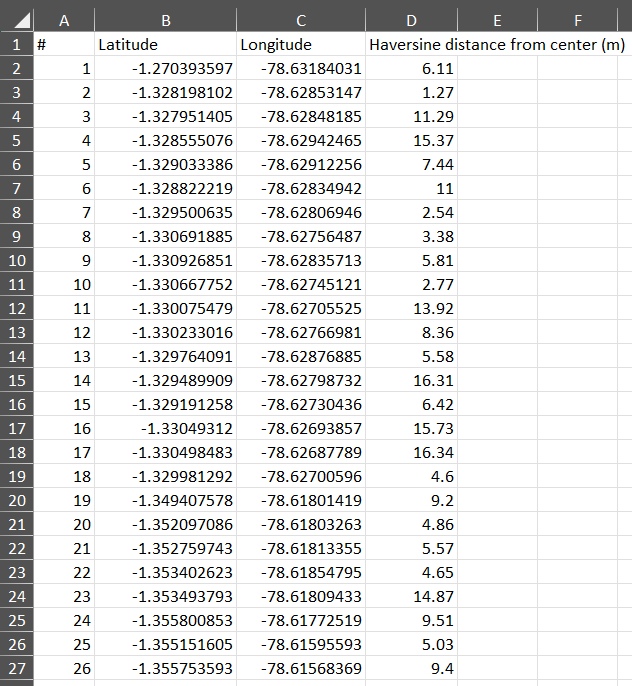
\includegraphics[width=0.5\textwidth]{chapters/III-resultados-y-discusion/resources/images/archivo-excel-georreferenciacion.png}
    \caption{Archivo de Excel con los datos georreferenciados para la comparación.}
    \label{fig:archivo-excel-georreferenciacion}
\end{figure}

Utilizando estos datos se creo un cluster de puntos georreferenciados en python, para ello se utilizó el algoritmo de K-Means, el cual
permite agrupar los puntos en clusters en función de su distancia. El código utilizado para la creación del cluster se muestra en el
Anexo \ref{apendix:script-cluster-python}. Utilizando el método del codo se determinó el número óptimo de clusters, el cual fue de 2 como
se muestra en la Figura \ref{fig:metodo-del-codo} en done se puede observar que el codo se encuentra en el punto 2.

% \begin{figure}[H]
%     \begin{minted}[fontsize=\footnotesize, linenos, breaklines, frame=single]{python}
import pandas as pd
import matplotlib.pyplot as plt
from sklearn.cluster import KMeans
import pygments as pg

df = pd.read_excel('geo-locations.xlsx', usecols='B:D', skiprows=0)
df.columns = ['latitude', 'longitude', 'distance']

# Elbow Method
def elbow_method(data):
    wcss = []
    for i in range(1, 11):
        kmeans = KMeans(n_clusters=i, max_iter=300)
        kmeans.fit(df[['latitude', 'longitude']])
        wcss.append(kmeans.inertia_)
    plt.plot(range(1, 11), wcss)
    plt.title('Método del Codo')
    plt.xlabel('Número de clusters')
    plt.ylabel('WCSS (Within Cluster Sum of Squares)')
    plt.show()

elbow_method(df)

# Cluster optimal number
numero_optimo_clusters = 2

# apply K-Means
kmeans = KMeans(n_clusters=numero_optimo_clusters, max_iter=300, random_state=42)
kmeans.fit(df[['latitude', 'longitude']])
df['cluster'] = kmeans.labels_

# Calc the mean distance of each cluster
distancias_medias_clusters = df.groupby('cluster')['distance'].mean()
print("Distancias medias de cada cluster:")
print(distancias_medias_clusters)

# Calc the mean of the mean distances of the clusters
media_de_las_medias = round(distancias_medias_clusters.mean(), 2)
print("Media de las distancias medias de los clusters:")
print(media_de_las_medias)

# Graph
plt.scatter(df['latitude'], df['longitude'], c=df['cluster'], cmap='viridis')
plt.title('Clusters de Puntos GPS')
plt.xlabel('Latitud')
plt.ylabel('Longitud')
plt.colorbar(label='Cluster')
plt.show()

\end{minted}


%     \caption{Script en Python para la creación de clusters de puntos georreferenciados.}
%     \label{apendix:script-cluster-python}
% \end{figure}

\begin{figure}[H]
    \centering
    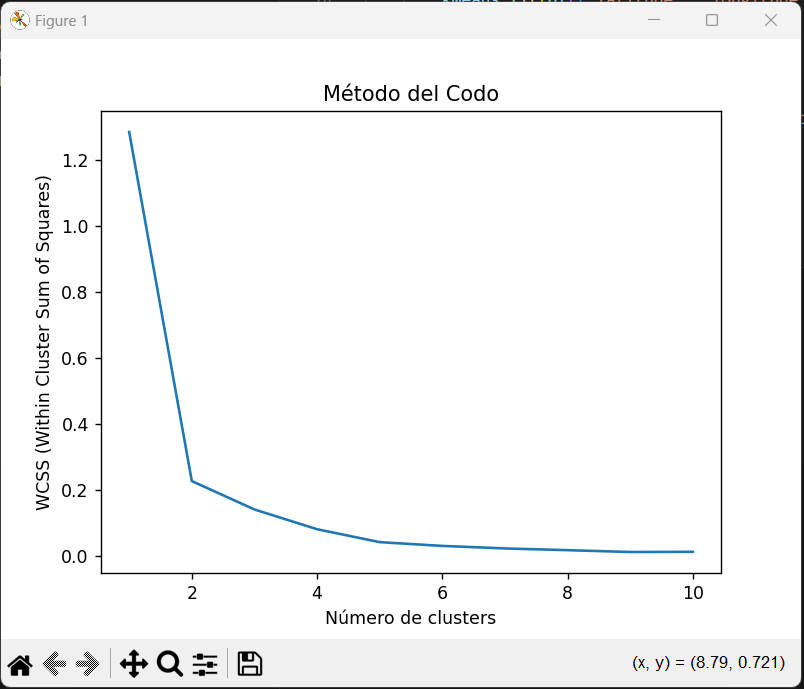
\includegraphics[width=0.5\textwidth]{chapters/III-resultados-y-discusion/resources/images/metodo-del-codo.png}
    \caption{Método del codo para determinar el número óptimo de clusters.}
    \label{fig:metodo-del-codo}
\end{figure}

El cluster resultante aplicando el algoritmo de K-Means se muestra en la Figura \ref{fig:cluster-georreferenciacion}.

\begin{figure}[H]
    \centering
    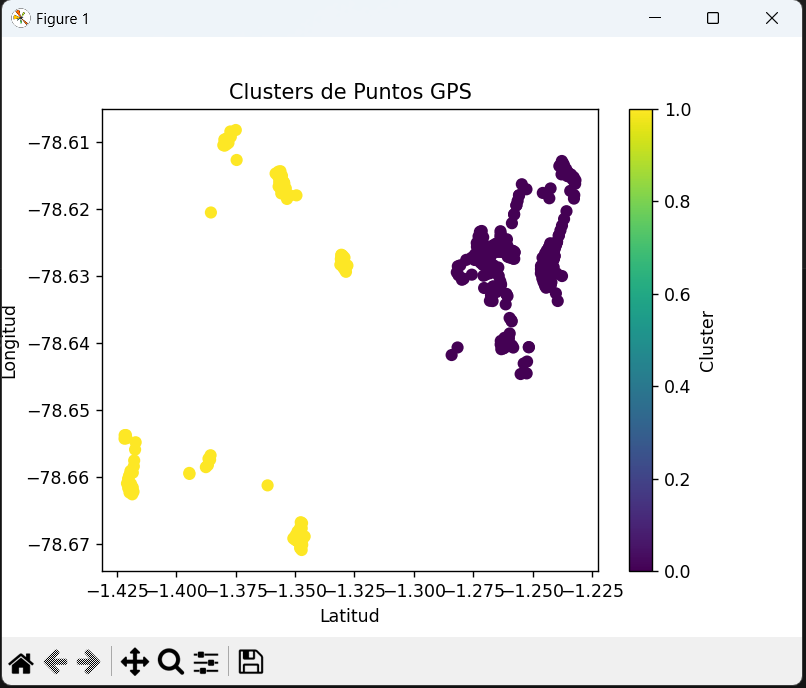
\includegraphics[width=0.5\textwidth]{chapters/III-resultados-y-discusion/resources/images/cluster-georreferenciacion.png}
    \caption{Cluster de puntos georreferenciados obtenidos mediante el algoritmo de K-Means.}
    \label{fig:cluster-georreferenciacion}
\end{figure}

Posteriormente se calculó la distancia media de cada cluster, así como la media de las distancias medias de los clusters. Los resultados
se muestran a continuación:

\begin{itemize}
    \item Distancias medias de cada cluster:
          \begin{itemize}
              \item Cluster 1: 6.32 m
              \item Cluster 2: 8.78 m
          \end{itemize}
    \item Media de las distancias medias de los clusters: 7.55 m
\end{itemize}

Estos resultados indican que la precisión media de los cluster es de 7.55 metros, Con la finalidad de obtener el intervalo de
confianza para esta media, se utilizó la Ecuación \ref{eq:ecuacion-intervalo-confianza}, donde:

\begin{itemize}
    \item IC = Intervalo de confianza
    \item M = Media de las distancias medias de los clusters
    \item ME = Margen de error
\end{itemize}

\begin{equation}
    IC = M \pm ME
    \label{eq:ecuacion-intervalo-confianza}
\end{equation}

El margen de error se calculó utilizando la Ecuación \ref{eq:ecuacion-margen-error}, donde:

\begin{itemize}
    \item ME = Margen de error
    \item Z = Valor crítico de la distribución normal estándar
    \item SE = Error estándar
\end{itemize}

\begin{equation}
    ME = Z \times SE
    \label{eq:ecuacion-margen-error}
\end{equation}

El error estándar se calculó utilizando la Ecuación \ref{eq:ecuacion-error-estandar}, donde:

\begin{itemize}
    \item SE = Error estándar
    \item $\sigma$ = Desviación estándar
    \item k = Tamaño de la muestra
\end{itemize}

\begin{equation}
    SE = \frac{\sigma}{\sqrt{k}}
    \label{eq:ecuacion-error-estandar}
\end{equation}


Sustituyendo los valores en las Ecuaciones \ref{eq:ecuacion-error-estandar} y \ref{eq:ecuacion-margen-error}, se obtiene:

\begin{itemize}
    \item Z = 1.96, con un nivel de confianza del 95\%
    \item $\sigma$ = 4.77
    \item k = 385
\end{itemize}

\begin{equation}
    SE = \frac{4.77}{\sqrt{385}} = 0.24
    \label{eq:ecuacion-resultado-error-estandar}
\end{equation}

\begin{equation}
    ME = 1.96 \times 0.24 = 0.47
    \label{eq:ecuacion-resultado-margen-error}
\end{equation}

Sustituyendo los valores en la Ecuación \ref{eq:ecuacion-intervalo-confianza} para el intervalo de confianza, se obtiene:

\begin{itemize}
    \item ME = 0.47
    \item M = 7.55
\end{itemize}

\begin{equation}
    IC = 7.55 \pm 0.47 = [7.08, 8.02]
    \label{eq:ecuacion-resultado-intervalo-confianza}
\end{equation}

Por lo tanto, se tiene que para un nivel de confianza del 95\%, el error de estimación de la precisión de los datos georreferenciados
se encuentra entre 7.08 y 8.02 metros con respecto al punto real de la ubicación.